%% *************************************************************************
%%
%% This is a derivative work of the RIT Space Exploration Standard defining
%% guidelines for content and formatting of project design documents.
%%
%% This document uses IEEEtran.cls, the official IEEE LaTeX class
%% for authors of the Institute of Electrical and Electronics Engineers
%% (IEEE) Transactions journals and conferences.
%%
%% *************************************************************************

\documentclass[conference]{IEEEtran} % http://www.ctan.org/pkg/ieeetran
\usepackage{blindtext} % enable placeholder text generator
\usepackage{graphicx} % enable toolbox for embedding figures and pictures
\usepackage{nomencl} % enable package for adding a list of variables and constants at the beginning, aka "nomenclature"
\usepackage{siunitx} % enable package for easily formatting units
\usepackage{hyperref} % enable package for cross-referencing figures, sections, references etc.
% how to use hyperref: http://www2.washjeff.edu/users/rhigginbottom/latex/resources/lecture09.pdf
\usepackage[T1]{fontenc} % change text encoding to make it more crisp
\usepackage{etoolbox} % enable conditionals for help text
\usepackage{booktabs} % make beautiful tables!

\title{Vegetation Density Mapping with Computer Vision Techniques using On-Board Image Processing}

\author{
   \IEEEauthorblockN{% This block is for author Names.
    Jeff~Maggio\IEEEauthorrefmark{1},
    Philip~Linden\IEEEauthorrefmark{2},
    T.J.~Tarazevits\IEEEauthorrefmark{3}
  }
  \IEEEauthorblockA{% This block is for the author Affiliations, aka department and university
    RIT Space Exploration, Rochester Institute of Technology \\ %\\ starts a new line
    Rochester, N.Y. \\
    Email:
    \IEEEauthorrefmark{1}jxm9264.rit.edu,
    \IEEEauthorrefmark{2}pjl7651@rit.edu,
    \IEEEauthorrefmark{3}tjt3085@rit.edu
  }
}
% page header for pages other than cover page
\markboth{Vegetation Density Mapping with Computer Vision}%
{Maggio \MakeLowercase{\textit{et al.}}: RIT Space Exploration}

\begin{document}
\maketitle%
% correct bad hyphenation here, separated by spaces
\hyphenation{explor-ation}

\begin{abstract}
    Advanced on-board image processing is a foundational component of a wide range of future space science and Earth observation missions.
    Extending these techniques to include computer vision opens the door to even more opportunities for science.
    It is critical to develop these techniques on low-cost, consumer hardware platforms so that the missions need not require expensive, specialized systems for every experiment.
    Demonstrating these systems are themselves opportunities for science as well.
\end{abstract}

\section{Introduction}
\label{sec:introduction}
  % The introduction is a place to give background and context before diving into the subject matter.
  % Establish context for the work you are about to propose and the main ideas of the proposition itself.

\IEEEPARstart{I}{mage} processing has long been a critical element of Earth observation and space science.
In recent years, the capabilities of inexpensive consumer electronics and computers have reached a point where advanced image processing can be performed on-board with lightweight, low-power computers.
This has opened the door for low-cost, rapid development experiment payloads and platforms such as high altitude balloons, drones, and small satellites.
Usually these platforms have limited communications bandwidth, so on-board processing may be used to significantly reduce the amount of data transferred back to ground without losing the information that the images contain.

Computer vision (CV) is defined as the automatic extraction, analysis and understanding of useful information from a single image or a sequence of images.
CV is the realm between image processing and computer science where useful information is identified, extracted, and interpreted from images without human input.
In addition to edge detection and other transforms applied to the pixel arrays directly, deeper and more abstract algorithms to interpret the contents of the images continue to mature in the field of machine learning.
These algorithms are trained, or iteratively tuned with a large set of data, to classify objects or cluster multivariate data from an arbitrary set of inputs.

Naturally, any implementation of image processing or CV for space science must be tested in a flight setting.
As this technilogy is developed, all tests are themselves opportunities for science.
This Project Definition Document considers the logistics of this development in addition to discussing a number of experiments that may be conducted as tests or end-user applications of on-board image processing and computer vision with low-cost, consumer electronics.

\section{Primary Objective}
\label{sec:primary-obj}
  % At the end of the day, whether the project ``succeeds'' or ``fails'' is judged against the objectives it sought to meet.
  % Note that results that contradict expectations/hypotheses are not failures if the scientific \& engineering methods are followed along the way.
  % Sometimes our expectations are wrong and that can be just as successful as getting data we thought we'd see.
  % What matters are what questions you intend to answer.
  % This is the main purpose or main goal the project hopes to achieve.

The SPEX Standard defines format and style guidelines for project documentation. The Project Design Document Standard controls these guidelines as applicable to young, exploratory ideas.

The ultimate goal of a PDD is to capture all ideas (including ones that are beyond our capability, interesting ideas, or things we just dont have time for, in addition to the ones that we actually work on and develop) and archive them such that if a student goes on coop or graduates, these ideas would not leave with them.

\begin{figure}
  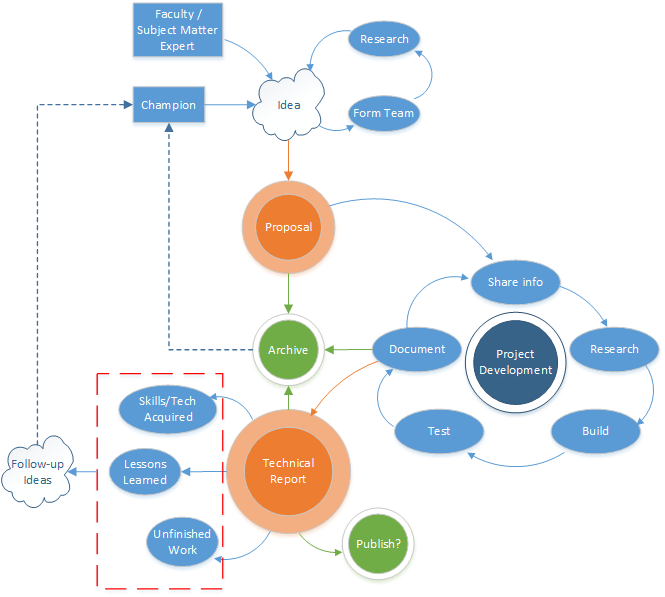
\includegraphics[width=\linewidth]{figs/project-life-cycle.png}
  \caption{A PDD is the first piece of documentation to be archived in the project life cycle. Since the life cycle can be iterative, a new design document may also refer to one or more previous SPPs.}
\label{fig:lifecycle}
\end{figure}

% \section{Secondary Objectives}
% \label{sec:secondary-obj}
% Secondary Objectives are lower priority or bonus objectives that are significant but not the main focus of the project. This template does not have secondary objectives.

\autoref{tab:long-example} lists a the relative level of detail expected of the documents written at each stage of a project's life.

\begin{table*}
% this table is too wide for the two-column format, so we let it expand across both columns
% we haven't told LaTeX where to put this so it'll find the best place.
    \caption{Relative detail expected at each stage of project development.}
    \centering
    \begin{tabular}{@{}llcc@{}}
        % READ THIS!! https://www.inf.ethz.ch/personal/markusp/teaching/guides/guide-tables.pdf
        \toprule % line on top external edge of table
        % Separate cells in a row with &, move to the next row with \\
        Document & Purpose & Contributors & Destination \\
        \midrule % line separating two internal rows
        Project Definition Document & To define the goals and requirements of a SPEX project. & 2--3 people & SPEX Archive \\
        Project Plans & Specific plans for when work is to be done (Gantt charts) & 2--3 people & Project Repository \\
        Design Reviews & To review designs before work is started. & 6--8 people & Project Repository \\
        Test Procedures & Specific instructions and data logs for tests. & 3--4 people & Project Repository \\
        User Manual & Instructions for future users of project deliverabels. & 3--4 people & Project Repository \\
        Posters \& Presentations & Materials for sharing projects with the public. & 5--6 people & Project Repository \\
        Technical Report & Final technical summary of work done and results. & 6 or more & SPEX Archive, Conferences \& Journals \\
        % LaTeX doesn't really like multi-line cell contents. Try to keep the text in each cell concise!
        \bottomrule
    \end{tabular}
\label{tab:long-example}
\end{table*}

\section{Benefit to SPEX}
\label{sec:benefit}
% One of the core values of SPEX is to provide opportunities for academic and professional growth for its members,
% and to challenge them with interesting projects.
% In this section, explain how the project would benefit SPEX members as students,
% space enthusiasts, and young professionals.

By writing design documents and familiarizing undergraduate and graduate students from any discipline with this type of approach and execution, SPEX members will be better equipped convey their ideas to others in a methodical and organized manner.
Ideally, an abundance of ideas and projects encapsulated in PDDs would outlive their respective authors and continue to sustain SPEX with valuable research opportunities invariant of individual members' absences due to co-ops or graduations.
Perhaps in the future, SPEX design documents may be used as baselines for grant applications and other funded research efforts.


% Below I have used subsections to identify key ideas in this section. These particular subsections are not required as part of the SPEX Standard, but serve as an example of using subsections in a text.

\subsection{Mindset}
\label{subsec:mindset}
Firstly, it gets people in the right mindset for thinking about what is important and what needs to be considered before taking off on a project.
Publishing a PDD imbues a sense of formality that hopefully makes its way into the level of seriousness and merit that is desirable for SPEX to pursue.

\subsection{Traceability}
\label{subsec:traceability}
Similarly, a PDD serves to provide the foundation for traceability in requirements and objectives to projects as they grow and change.
This prevents blockers such as feature creep, rabbit holes, and spun tires, and hopefully prevents good projects from dying by getting too off track.

\subsection{Accessibility}
\label{subsec:plug-n-play}
  % Note below that LaTeX uses weird formatting when it comes to quotation marks.
  % The style below is correct to display forward quotes `` at the start of the phrase and backquotes '' at the end.

Having a ``plug-and-play'' template is the first step to learning how to one's own PDD\@.
It removes a major barrier of starting from scratch, providing example content to which one could refer when creating their own.
\LaTeX{} may prove to be daunting for some people, but it is arguably better to encourage people to learn LaTeX than to rely on something like Microsoft Word~\cite{lamp94}.

\section{Implementation}
\label{sec:implementation}
  % What path do you anticipate the project to take?

In the ideal case, every project begins with a design document.
That design document gets sent around to SPEX members (and non-members) to draw support and build a team.
Research and work takes place, documented along the way until  an ending point is reached (e.g.\ project completion, end of the semester, team attrition, etc.).

At the end of the project (or end of semester, whichever comes first), the team writes a report of the project with what they did, if it was successful, and recommendations for future projects.
A future SPEX member might pick up where the last paper left off, and the cycle repeats.

\subsection{Deliverables}
\label{subsec:deliverables}
  % When all is said and done, what will you have to show for it?
  % Examples: Hardware, software, poster, ImagineRIT demo, presentations, technical papers...
Physical or intellectual property may constitute a project's deliverables.
Test articles, test stands, and other hardware, software, as well as posters, presentations or other reports are all valid deliverables.
Not all deliverables may be known at the time of writing a PDD, but at least several key deliverables should be identified at the start of a project.
This helps guide the final outcome and is a fundamental part of a project's life cycle.

\subsection{Milestones}
\label{subsec:milestones}
  % Be as detailed as you can, but it's okay if there are unknowns.
  % At the very least, specify how many semester you expect the project to take until it reaches completion.
Deadlines and milestones provide clear goals from which timelines and schedules may be developed, and also set up a project for a series of ``sanity checks'' along the project's development cycle.
Early on, these milestones include design reviews on system and subsystem levels.
Later, milestones are usually important tests or experiments.
Events such as ImagineRIT may also serve as milestones to mark a project's development progress or completion.

A notional timeline is shown in \autoref{tab:short-example}.

\begin{table}[hb!]
    % the "h" in these brackets tells LaTeX to put the table Here. Try [t] for top and [b] for bottom,
    % or [hbp] for "here, or if you can't do that put it at the bottom of the page, or if you can't do that put it on its own page.
    % Here we've also used an "!" to yell at LaTeX to DO THIS OR ELSE!
    \caption{Notional timeline of Project Milestones.}
    \centering
    \begin{tabular}{@{}cll@{}}
    % the letters here ^^^^ designate the columns.
    % (l=left align, c=center, r=right align)
    % the weird @{} thingies tell LaTeX to not have left-right padding between cells
    % so cells butt up right against the edge
    \toprule
    Phase & Task & Duration \\
    \midrule
    1 & Review existing designs and materials & 2 weeks or less\\
    2 & Subsystem development & 6 weeks \\
      & Order PCB design and/or assembly & 6 weeks \\
      & Review changes and order materials & 2 weeks or less\\
      & Testing of individual subsystems & 2 weeks \\
    3 & System assembly & 1 week  \\
    4 & System testing & 2 weeks  \\
    5 & Generate documentation and delivery to SPEX & 1 week  \\
    \bottomrule
    \end{tabular}
\label{tab:short-example}
\end{table}

\section{Externalities}
  % Things not directly related to the work or outcomes, but related to the project as a whole.
\subsection{Prerequisite Skills}
  % Which skills do team members need to have before work can start (not including skills that will be learned ``on the job'')?
It is obvious that team members will learn certain skills as a project progresses, but there are always some tasks that require a minimum skill level to provide meaningful contributions to a project's development.
These prerequisite skills are best identified by examining past projects and discussing the project with faculty or subject matter experts.
It is strongly recommended to be conservative in skill estimation.
Underestimate team member skill levels and overestimate the challenge.
Many projects have failed because the team overestimated their own abilities or underestimated the difficulty of their project.

\subsection{Funding Requirements}
  % Estimate costs that would be needed to meet objectives.
Like prerequisite skills, it is wise to overestimate the cost of components, materials and other resources that a project requires.
For physical projects, costs may be estimated by benchmarking the costs of similar systems or determining a representative bill of materials and using the aggregate cost of its items.

\subsection{Faculty Support}
  % Identify faculty that will be involved (or would need to be involved) to meet objectives.
  % Note that if a professor is the Principal Investigator (P.I.) for a project, there still needs to be a student as the SPEX Project Champion.
Support from university faculty is almost always essential to a project's success.
Faculty provide not only guidance and subject matter expertise, but may also connect a team with resources and networking opportunities.
SPEX projects do not require faculty support, but it is highly recommended to identify professors with an interest or expertise in a project as early as possible.

\subsection{Long-Term Vision}
\label{sec:vision}
As SPEX student members get more experience writing these papers, the group will build a library of meaningful work and be able to save it in an organized manner.
Knowledge will be preserved and easily shared.
Perhaps Project Design Document could eventually get published, in a journal or otherwise\ldots

\section*{Acknowledgements}
The author would like to thank Dr.~Bill Destler and Rebecca Johnson for being exemplary humans, Anthony Hennig for founding RIT Space Exploration, and all the SPEX members that continue to invest their time and energy into the pursuit of space exploration.

\bibliographystyle{IEEEtran}
\bibliography{sample-with-examples}

\onecolumn
\appendices{}
\section{Project Life Cycle}
\begin{figure}[h]
  \centering
  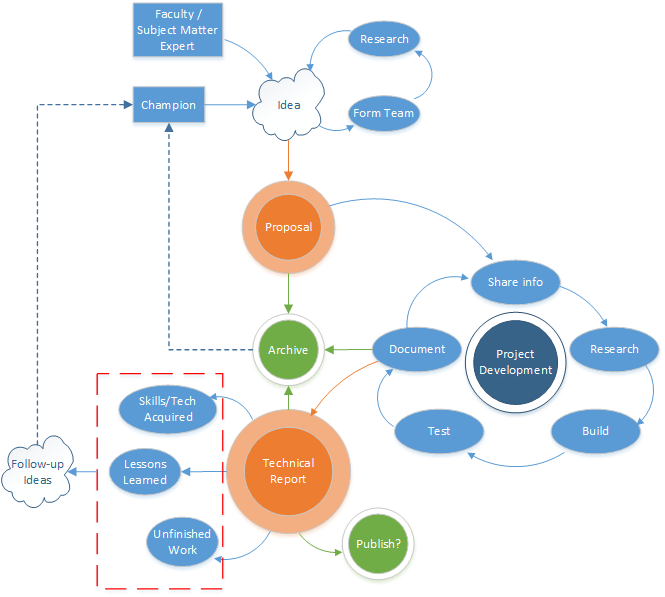
\includegraphics[]{figs/project-life-cycle.png}
  \caption{Enlarged version of the diagram in \autoref{fig:lifecycle}.}
\end{figure}

\end{document}
